\section{Proposed FPGA implementation of SWIFT}
\label{Sec:FPGA}

In this section we describe the proposed FPGA implementation of the SWIFT algorithm as described by Equation \ref{eq:X_n_X_n1}. As seen in Figure \ref{fig:SWIFT_structure}, the fundamental computation unit hereafter referred to as a `SWIFT slice' consists of a complex multiplier, a complex adder and a single delay element. When implementing this function inside a FPGA, a sample $x(n)$  needs to pass through the multiplier and be available at the input of the adder when the next sample $x(n+1)$ comes in. On an FPGA, the complex multiplier and complex adder are implemented using the floating point add (FPADD) and floating point multiply (FPMUL) library functions available in the FPGA design tool. The complex floating point adder requires two FPADD operators, while the complex floating point multiplier requires four FPMUL and two FPADD operators. Thus a single `SWIFT slice' requires a total of 4 floating point adders and 4 floating point multipliers. The organization of the library functions to achieve the functionality of the `SWIFT slice' is shown in Figure \ref{fig:SWIFT_unit}.

\begin{figure}[tbp]
\centering
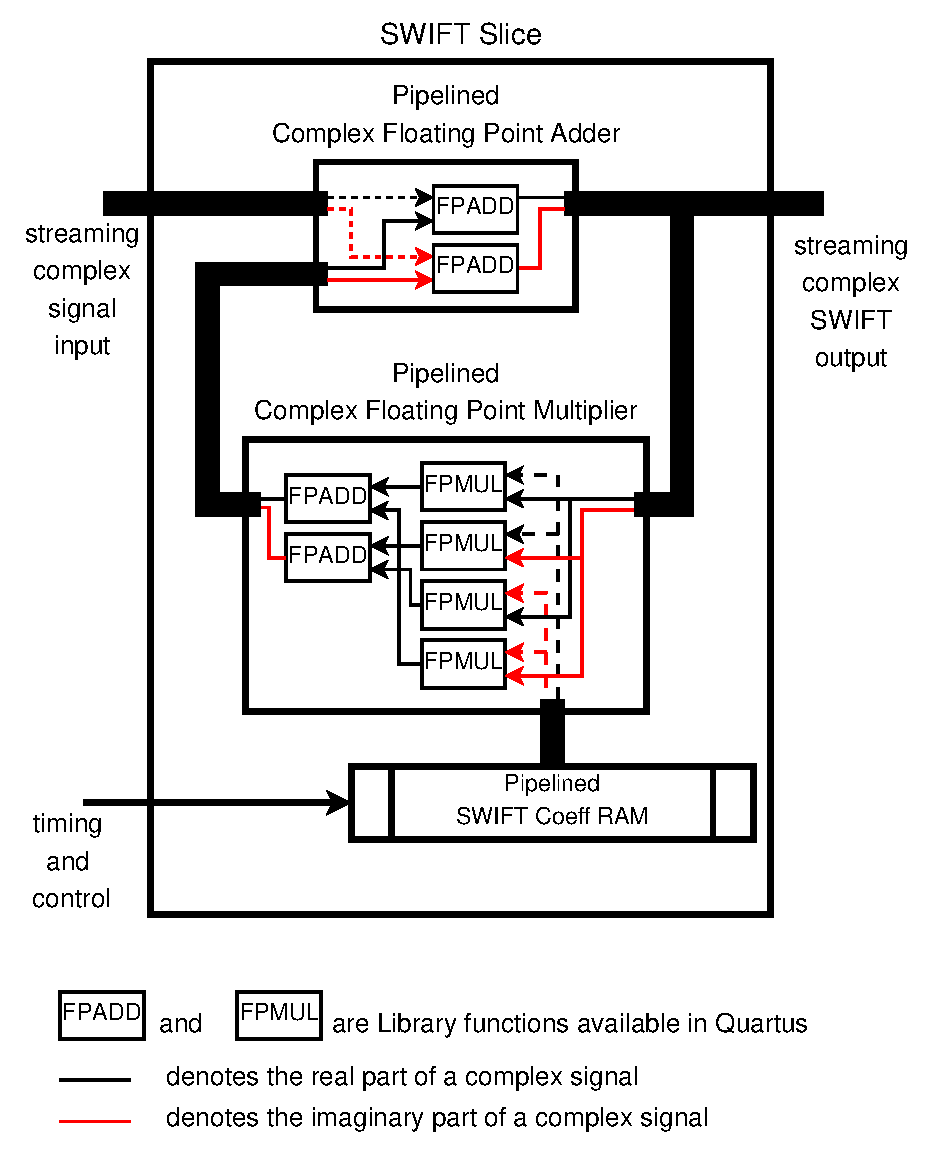
\includegraphics[width=0.85\columnwidth]{Figures/fig_SWIFT_slice.eps}
\caption{Block diagram of SWIFT slice}
\label{fig:SWIFT_unit}
\end{figure}

An important characteristic of the hardware library functions FPADD and FPMUL is their latency measured in terms of the number of clock cycles required to produce a valid output after the inputs are stable. These latencies are non-zero and this implies that a sample $x[n-1]$ presented at the input of the `SWIFT unit' will take some finite number of clock cycles to pass through all the modules and generate a value for $e^{-1/\tau}e^{j\omega}X_{n-1}(\omega)$ that can be added to the next sample $x[n]$.

If the the adder and the multiplier have latencies of $cyc_{fa}$ $cyc_{fm}$, and the data samples are presented at the input at a rate of $Srate_{din}$ Msps, the minimum frequency of the clock $f_{SWIFT}$ in MHz required to run the SWIFT slice is given by
\begin{equation}
\label{eq:swift_freq}
f_{SWIFT} \geq (cyc_{fa} + cyc_{fm} + cyc_{fa}) \times srate_{din} 
\end{equation}. 

Equation \ref{eq:swift_freq} implies that SWIFT slice needs to run at a higher frequency than the sampling frequency of the incoming signal. The higher frequency of the SWIFT clock ensures that a data sample being processed by the SWIFT algorithm, passes through the complex adder and multiplier and is available back at the input of the complex adder before the next sample comes in. Figure \ref{fig:SWIFT_slice_waveform} illustrates the timing relation between the signals inside a SWIFT unit. An interesting consequence of this relation is that when the left and right sides in Equation \ref{eq:swift_freq} are equal, a separate storage element to delay the computed value of $X_n(\omega)$ is not required, as the delay through the computation units achieves this functionality.

\begin{figure*}
\centering
\begin{tikztimingtable}
  	sample clock  & 9.5L 3{9.5C} 9.5L \\
  	SWIFT clock   & 95{0.5C}\\
  	sample  	  & [timing/text format={\large}]9.5D{x[n-1]} N(S1) {} 19D{x[n]} {} 19D{x[n+1]}\\
 	\textbf{Adder} \\
  	FPADD out  	  & [timing/text format={\large}]16.5D{$X_{n-1}(\omega_x)$} N(S2) {} N(FA1) 19D{$X_n(\omega_x)$} {} 12D{$X_{n+1}(\omega_x)$} \\
    \textbf{SWIFT RAM} \\
   	SWIFT Coeff	  & [timing/text format={\large}]47.5D{($\tau_x, \omega_x)$} \\
    \textbf{Mutliplier} \\
   	FPMUL out  	  & [timing/text format={\large}]21.5D{$Dmul_{n-1}(\omega_x)$} {} N(FM1) 19D{$Dmul_n(\omega_x)$} {} 7D{} \\
    FPADD out  	  & [timing/text format={\large}]28.5D{$Dadd_{n-1}(\omega_x)$} {} N(FA2) 19D{$Daddr_n(\omega_x)$} {} D{} \\ \\ 	
	\extracode
  	\tablerules
	\begin{pgfonlayer}{background}
    	\vertlines [help lines] {9.5,16.5,21.5,28.5};
        
        \node [anchor = mid ] at (13,-5){\small $cyc_{fa}$};
        \draw [<->] (9.5,-6) -- (16.5,-6);
        
        \node [anchor = mid ] at (19,-13){\small $cyc_{fm}$};
        \draw [<->] (16.5,-14) -- (21.5,-14);
        
        \node [anchor = mid] at (25,-19){\small $cyc_{fa}$};
        \draw [<->] (21.5,-20) -- (28.5,-20);
  	\end{pgfonlayer}
\end{tikztimingtable}
\caption{SWIFT slice timing waveform for a frequency $\omega_x$}
\label{fig:SWIFT_slice_waveform}
\end{figure*}


In a FFT computation the frequency resolution is a function of the sampling rate and the number of points in the FFT. However for the SWIFT the frequency resolution can be configured to be independent of the sampling frequency. If the system is required to compute a Discrete Fourier Transform in the frequency range $f_{lo}$ to $f_{hi}$ with a frequency resolution of $\delta f$, such that
\begin{equation}
f_{hi} - f_{lo} = M \times \delta f
\end{equation}
where $M$ is an integer
The normalised frequencies are given by $\omega_{lo}  = 2\pi f_{lo}/f_s$ and $\omega_{hi} = 2\pi f_{hi}/f_s$. 
It may be noted from Equation \ref{eq:X_n_X_n1} that given a discrete sample $x[n]$, computation of the SWIFT value for the frequency $f_m = f_{lo} + m\delta f$, where $m \in [0,M)$, is dependent only on the SWIFT coefficient $C_m = e^{-1/\tau_m} e^{j\omega_m}$ and the previous SWIFT value. The computation does not depend on the final or intermediate SWIFT value for any other frequency as is the case in a radix-2 or a radix-4 FFT. $M$ SWIFT slices, can therefore be stacked in parallel and fed by a single data input sample to compute SWIFT values over the complete frequency range. 

This arrangement is however inefficient in its utilization of the hardware resources. This is because while the FPADD and FPMUL library functions have finite latencies, they can be time multiplexed to perform addition and multiplications on distinct inputs every clock cycle without affecting the result in any other clock cycle. 
Thus, instead of having $M$ SWIFT slices stacked in parallel each working with a single SWIFT coefficient $C_m$, $m \in [0,M)$ to generate the SWIFT value for a single frequency bin, we have each slice working with a set of SWIFT coefficients. The relation between the number of coefficients in each set $l$, the number of slices $s$ and the total number of frequency bins in the DFT $M$ is given by 
\begin{equation}
\label{eq:tdm_slices}
M = s \times l.
\end{equation}
Thus slice$1$ works with a set of coefficients $\{C_0, C_1 \ldots C_{l-1}\}$, slice$2$ works with a set of coefficients $\{C_l, C_{l+1} \ldots C_{2l-1}\}$ and so on, with the final slice$s$ working with a set of coefficients $\{C_{(s-1)l}, C_{(s-1)l+1}, \ldots C_{M-1}\}$ in a time multiplexed manner. 
For a single data sample $x[n]$, the SWIFT coefficients in a set are presented at the input of the complex floating point multiplexer one per clock cycle. A timing diagram illustrating this behaviour is shown in Figure \ref{fig:SWIFT_slice_time_share_waveform}. As seen in the timing diagram, after a latency equal to $cyc_{fm} + cyc_{fa}$ clock cycles, the data is available at the output of the complex floating point multiplier. At this instant the next sample $x[n+1]$ is available at the input of the adder and the correct SWIFT value $X_n(\omega)$ is generated after $cyc_{fa}$ clock cycles and it goes into the complex floating point multiplier, where the coefficients are again presented starting with the first coefficient in the set. This scheme is illustrated in the timing diagram in Figure \ref{fig:SWIFT_slice_time_share_waveform}.

The maximum number of coefficients in a slice is determined by the relation between $f_{SWIFT}$ and $srate_{din}$ given by Equation \ref{eq:swift_freq}. 

\begin{figure}[tbp]
\centering
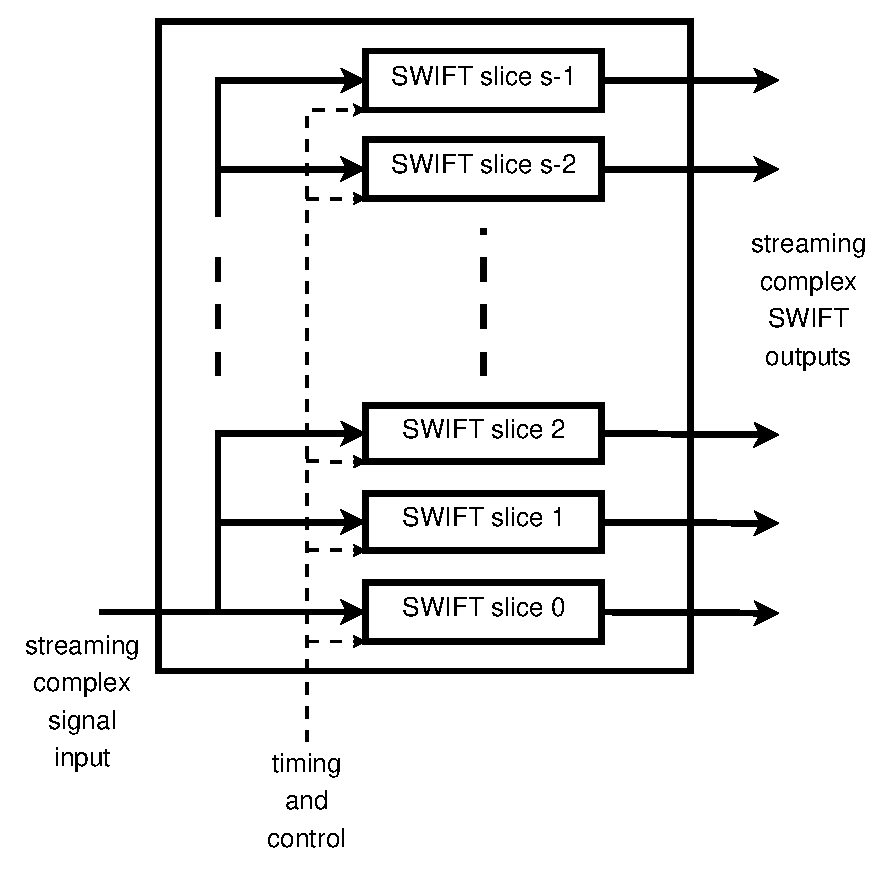
\includegraphics[width=\columnwidth]{Figures/fig_SWIFT_computation.eps}
\caption{Internal organization of SWIFT computation block}
\label{fig:SWIFT_slices}
\end{figure}



\begin{figure*}
\centering
\begin{tikztimingtable}
  	sample clock  	& 9.5L 3{9.5C} 9.5L \\
  	SWIFT clock   	& 95{0.5C}\\
  	sample  		& [timing/text format={\large}]9.5D{x[n-1]} N(S1) {} 19D{x[n]} {} 19D{x[n+1]}\\
 	\textbf{Adder} \\
  	FPADD out  		& [timing/text format={\large}]16.5D{$X_{n-1}(\omega_x)$} N(S2) {} N(FA1) 19D{$X_n(\omega_x)$} {} 12D{$X_{n+1}(\omega_x)$} \\
    \textbf{Mutliplier} \\
   	FPMUL out  		& [timing/text format={\large}]21.5D{$Dmul_{n-1}(\omega_x)$} {} N(FM1) 19D{$Dmul_n(\omega_x)$} {} 7D{} \\
    FPADD out  		& [timing/text format={\large}]28.5D{$Dadd_{n-1}(\omega_x)$} {} N(FA2) 19D{$Daddr_n(\omega_x)$} {} D{} \\ \\ 	
	\extracode
  	\tablerules
	\begin{pgfonlayer}{background}
    	\vertlines [help lines] {9.5,16.5,21.5,28.5};
        \node [anchor = mid ] at (13,-5){\small $cyc_{fa}$};
        \draw [<->] (9.5,-6) -- (16.5,-6);
        \node [anchor = mid ] at (19,-9){\small $cyc_{fm}$};
        \draw [<->] (16.5,-10) -- (21.5,-10);
        \node [anchor = mid] at (25,-15){\small $cyc_{fa}$};
        \draw [<->] (21.5,-16) -- (28.5,-16);
  	\end{pgfonlayer}
\end{tikztimingtable}
\caption{SWIFT slice timing waveform with time sharing}
\label{fig:SWIFT_slice_time_share_waveform}
\end{figure*}


required as well as  as shown in Figure \ref{fig:M_swift_slices}

\begin{figure}[tbp]
\centering
\includegraphics[width=\columnwidth]{Figures/fig_FPGA_system_diagram.eps}
\caption{System diagram of an FPGA implementation of the SWIFT algorithm}
\label{fig:FPGA_system_design}
\end{figure}

